\documentclass[pdf,table]{beamer}
\usepackage{graphicx,hyperref,pdfpages}
\usepackage{tikz}
\usepackage{textpos}
\usepackage{longtable}
\usepackage{listings}
\usepackage{color}
\usepackage{listings}
\usepackage{color}
\usepackage[style=numeric,backend=biber]{biblatex}
%
\usetikzlibrary{arrows}
\usetikzlibrary{positioning,chains,fit,shapes,calc}
\usetikzlibrary{mindmap}
\usetikzlibrary{shapes.multipart}
\usetikzlibrary{decorations.text}
%
\addbibresource{../CST4025.bib}
\setbeamertemplate{bibliography item}{\insertbiblabel}
%
%defin colours
\definecolor{codegreen}{rgb}{0,0.6,0}
\definecolor{codegray}{rgb}{0.5,0.5,0.5}
\definecolor{codepurple}{rgb}{0.58,0,0.82}
\definecolor{backcolour}{rgb}{0.95,0.95,0.92}
\definecolor{delim}{rgb}{20,105,176}



\lstdefinelanguage{CTO}{
	keywords={abstract, asset, by, concept, default, enum, event, identified, Integer, o, participant, String, transaction },
	comment=[l]{//},
	comment=[s]{/*}{*/},
	string=[b]",
	sensitive=true,
}

\lstdefinelanguage{ACL}{
	keywords={transaction,condition,rule,description,participant,operation,resource,action,ALLOW,READ,ALL,CREATE,UPDATE,DELETE,ANY,DENY},
	comment=[l]{//},
	comment=[s]{/*}{*/},
	string=[b]",
	sensitive=true,
}

%define Javascript language
\lstdefinelanguage{JavaScript}{
keywords={typeof, new, true, false, catch, function, return, null, catch, switch, var, if, in, while, do, else, case, break},
keywordstyle=\color{blue}\bfseries,
ndkeywords={class, export, boolean, throw, implements, import, this},
ndkeywordstyle=\color{darkgray}\bfseries,
identifierstyle=\color{black},
sensitive=false,
comment=[l]{//},
morecomment=[s]{/*}{*/},
commentstyle=\color{purple}\ttfamily,
stringstyle=\color{red}\ttfamily,
morestring=[b]',
morestring=[b]"
}
%define json language
\colorlet{punct}{red!60!black}
\definecolor{background}{HTML}{EEEEEE}
\definecolor{delimiter}{RGB}{20,105,176}
\colorlet{numb}{magenta!60!black}

\lstdefinelanguage{json}{
    numbers=left,
    numberstyle=\scriptsize,
    stepnumber=1,
    numbersep=8pt,
    showstringspaces=false,
    breaklines=true,
    frame=lines,
    backgroundcolor=\color{background},
    literate=
     *{0}{{{\color{numb}0}}}{1}
      {1}{{{\color{numb}1}}}{1}
      {2}{{{\color{numb}2}}}{1}
      {3}{{{\color{numb}3}}}{1}
      {4}{{{\color{numb}4}}}{1}
      {5}{{{\color{numb}5}}}{1}
      {6}{{{\color{numb}6}}}{1}
      {7}{{{\color{numb}7}}}{1}
      {8}{{{\color{numb}8}}}{1}
      {9}{{{\color{numb}9}}}{1}
      {:}{{{\color{punct}{:}}}}{1}
      {,}{{{\color{punct}{,}}}}{1}
      {\{}{{{\color{delimiter}{\{}}}}{1}
      {\}}{{{\color{delimiter}{\}}}}}{1}
      {[}{{{\color{delimiter}{[}}}}{1}
      {]}{{{\color{delimiter}{]}}}}{1},
}
%\lstdefinelanguage{json}{
%    numbers=left,
%    numberstyle=\scriptsize,
%    stepnumber=1,
%    numbersep=8pt,
%    showstringspaces=false,
%    breaklines=true,
%    frame=lines,
%    backgroundcolor=\color{backcolour},
%    literate=
%     *{\{}{{{\color{delim}{\{}}}}{1}
%      {\}}{{{\color{delim}{\}}}}}{1}
%      {[}{{{\color{delim}{[}}}}{1}
%      {]}{{{\color{delim}{]}}}}{1},
%}



\lstdefinestyle{mys}{
	backgroundcolor=\color{backcolour},
	commentstyle=\color{codegreen},
	keywordstyle=\color{magenta},
	stringstyle=\color{codepurple},
	numberstyle=\color{codegray},
	basicstyle=\ttfamily\tiny,
	breakatwhitespace=false,
	breaklines=true
	captionpos=b,
	keepspaces=true,
	numbers=left,
	numbersep=5pt,
	showspaces=false,
	showstringspaces=false,
	showtabs=false,
	tabsize=2}
\lstset{style=mys}



\tikzset{every matrix/.style={ampersand replacement=\&,column sep=1.75cm,row sep=2cm},
		BTWMat/.style={ampersand replacement=\&, column sep=0.75cm,row sep=1cm},
		eulerMat/.style={ampersand replacement=\&,column sep=1.1cm,row sep=2cm},
		vertexHighlight/.style={circle,fill=red!80,inner sep=.1cm,text=white},
		vertex/.style={circle,fill=blue!80,inner sep=.1cm,text=white},
		bank/.style={rectangle,fill=blue!50,inner sep=0.1cm,text=black!80}
		edge/.style={--,line width=2pt},
		Dedge/.style={->,line width=2pt},
		DedgeT/.style={->,line width=1pt},
		BiEdge/.style={<->,line width=2pt},
		BiEdgeT/.style={BiEdge,line width=1pt},
		edgeHighlight/.style={--,line width=2pt,color=red},
		loop/.style={min distance=10mm, line width=2pt},
		loopT/.style={min distance=-10mm, line width=1pt},
		label/.style = { rectangle, rounded corners, draw,
		                 minimum width = 2em, fill = yellow!50,
		                 text = red, font = \tiny\bfseries },
		labelT/.style = { circle, draw, line width=1pt,
		                 minimum width = 1em, fill = yellow!50,
		                 text = red, font = \tiny\bfseries },
		every node/.style={align=center}}



\newcommand{\cwideadline}{3$^{rd}$ November 2019}
\newcommand{\cwiideadline}{5$^{th}$ January 2020}
%\newcommand{\cwiiideadline}{31$^{st}$ March 2017}
%\newcommand{\cwiiideadline}{15$^{th}$ April 2018}
\newcommand{\resitdeadline}{1$^{st}$ August 2020}
\newcommand{\deferraldeadline}{1$^{st}$ August 2020}
\newcommand{\deferraldeadlineMay}{1$^{st}$ May 2020}
\newcommand{\moduleCode}{CST4025}
\newcommand{\moduleLeader}{Dr Ian Mitchell }
\newcommand{\theauthor}{Dr Ian Mitchell }
\newcommand{\academicyear}{2019-20}
\newcommand{\email}{i.mitchell@mdx.ac.uk}
\newcommand{\moduleTitle}{Blockchain Development}
\newcommand{\office}{T108}
\newcommand{\officehours}{Autumn \& Winter Terms: Tuesdays 1515-1615hrs; and, Wednesdays 1415-1515hrs}
\newcommand{\tel}{0208-411-6014}
\newcommand{\deptName}{Computer Science}
%\newcommand{\officehours}{Friday 1100\--1300hrs Autumn Term \\ Thursday 1400\--1600hrs Winter Term}
%\newcommand{\officehours}{Autumn Term: Mondays 1300\--1500hrs \\ Winter Term: Thursdays 1400\--1600hrs

\def\bitcoinA{%
  \leavevmode
  \vtop{\offinterlineskip %\bfseries
    \setbox0=\hbox{B}%
    \setbox2=\hbox to\wd0{\hfil\hskip-.03em
    \vrule height .3ex width .15ex\hskip .08em
    \vrule height .3ex width .15ex\hfil}
    \vbox{\copy2\box0}\box2}}



%
\mode<presentation>{
\usetheme{Madrid}
\usecolortheme{beaver}
}
%
\newcommand{\theweek}{6}
\renewcommand{\theequation}{\theweek.\arabic{equation}}

\title[\moduleCode:L\theweek]{\moduleTitle \\ Week: \theweek \\ Title: Node.js and TX} 
\institute[]{\includegraphics[scale=0.25]{../../../logo/mdxSmall} \\ Middlesex University, \\Dept. of Computer Science, \\London}
\author[\textcopyright \email]{\moduleLeader}
\date{\today}




\begin{document}
	\begin{frame}
		\titlepage
	\end{frame}


\addtobeamertemplate{frametitle}{}{%
\begin{textblock*}{100mm}(.94\textwidth,-0.85cm)
\includegraphics[scale=0.1]{../../../logo/transparent}
\end{textblock*}}

	\begin{frame}{Lecture Aims}
		\begin{block}{Aims}
			There are four components to hyperledger's  composer playground:
			\begin{enumerate}
				\item Data
				\item Access
				\item Logic
				\item Query
			\end{enumerate}
			After last week's introduction to Node.js, this week we will investigate how node.js can be applied to fit the logic of a blockchain application, and essentially work towards transaction completion.
		\end{block}
	\end{frame}

	\begin{frame}{Lecture Objectives}
		\begin{block}{Knowledge}
			\begin{itemize}
				\item Retrieving registers
				\item Updating registers
				\item Transaction Completion
				\item Composer API
			\end{itemize}	
		\end{block}
	\end{frame}

\begin{frame}{Hyperledger}{Composer}
	\begin{itemize}
		\item ACL
		\item CTO
		\item Javascript ES6
			\begin{itemize}
				\item ECMAScript 2015
				\item ECMA is a an organisation for the standardisation of information and communication systems
				\item ECMA was founded in 1961
				\item \url{www.ecma-international.org}
			\end{itemize}
		\item Netscape submitted Javascript to ECMA for standardisation
		\item Result ECMAScript
		\item ES1 - 1997
		\item ES6 - 2015
		\item ES8 - 2017
	\end{itemize}
\end{frame}

\begin{frame}{Hyperledger Composer API}{Registry Classes}
	\begin{itemize}
		\item AssetRegistry
		\item ParticipantRegistry
		\item IdentityRegistry
		\item TransactionRegistry
		\item Historian
	\end{itemize}
\end{frame}

\begin{frame}{Registry functions}
	\begin{itemize}
		\item Add one or more items
		\item Update one or more items 
		\item Remove one or all items
		\item Get one or all items
		\item Check if an item exists
		\item Resolve one or all items
	\end{itemize}
\end{frame}

\begin{frame}[fragile]{Transactions}{lib/logic.js}
	\begin{block}{header}
	\begin{verbatim}
		/**
		* Create a transaction 
		* @param {namespace.TransactionName} tx - further comment
		* @transaction
		*/
		\end{verbatim}
	\end{block}
\end{frame}

\begin{frame}[fragile,allowframebreaks]{Trader \footnote{adapted from \url{hyperledger.org} tutorials}}{CTO}
	\lstinputlisting[language=CTO]{t5/models/sample.cto}
\end{frame}

\begin{frame}[fragile,allowframebreaks]{Trader \footnote{adapted from \url{hyperledger.org} tutorials}}{ACL}
	\lstinputlisting[language=ACL]{t5/permissions.acl}
\end{frame}

\begin{frame}[fragile,allowframebreaks]{Trader \footnote{adapted from \url{hyperledger.org} tutorials}}{JS}
	\lstinputlisting[language=JavaScript,lastline=12]{t5/lib/sample.js}
\end{frame}



\begin{frame}{Compare CTO and JS}
	\begin{columns}[T]
		\begin{column}{0.48\textwidth}
			\lstinputlisting[language=CTO,numbers=none]{t5/models/sample.cto}
		\end{column}
		\begin{column}{0.48\textwidth}
			\lstinputlisting[language=JavaScript,lastline=12,numbers=none]{t5/lib/sample.js}
		\end{column}
	\end{columns}	
\end{frame}


\begin{frame}{Traders Example}
	\begin{columns}[T]
		\begin{column}{0.5\textwidth}
			\lstinputlisting[language=JavaScript,lastline=12]{t5/lib/sample.js}
		\end{column}
		\begin{column}{0.5\textwidth}
			\small
			\begin{itemize}
				\item 1-5 comments
				\item @param has namespace, followed by transaction name
				\item @transaction identifies the following function as a TX
				\item 6 function name is unique and does not match transaction name. It does take transaction as a parameter.
				\item 7 changes ownership, owner replaced by newOwner
				\item 8 get Commodity registry
				\item 9 update Commodity registry
			\end{itemize}
		\end{column}
	\end{columns}	
\end{frame}

\begin{frame}{Traders Example}{Output Trader}
	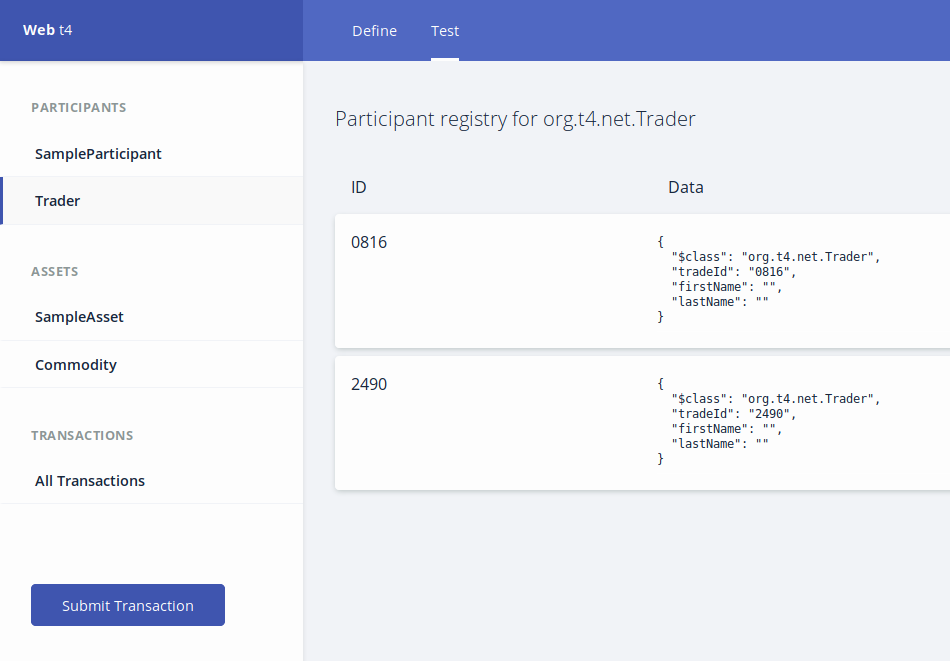
\includegraphics[scale=0.35]{t4-Trader}
\end{frame}

\begin{frame}{Traders Example}{Output Commodity}
	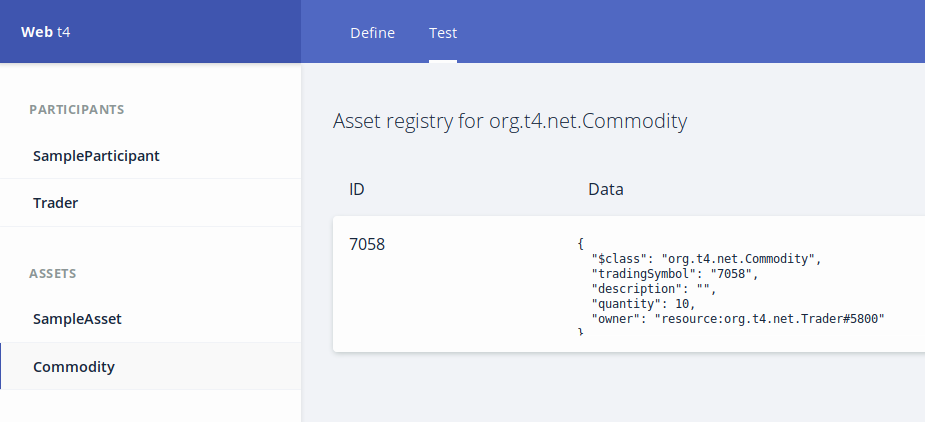
\includegraphics[scale=0.35]{t4-Commodity}
\end{frame}

\begin{frame}[fragile]{Traders Comparison?}
	\begin{columns}[T]
		\begin{column}{0.40\textwidth}
			{\bf Traders}	
			\begin{lstlisting}[language=json]
{
  "$class": "org.t4.net.Trader",
  "tradeId": "0816",
  "firstName": "",
  "lastName": ""
}		
{
  "$class": "org.t4.net.Trader",
  "tradeId": "2490",
  "firstName": "",
  "lastName": ""
}
			\end{lstlisting}
		\end{column}

		\begin{column}{0.58\textwidth}
			{\bf Commodity}
			\begin{lstlisting}[language=json]
{
  "$class": "org.t4.net.Commodity",
  "tradingSymbol": "7058",
  "description": "",
  "quantity": 10,
  "owner": "resource:org.t4.net.Trader#5800"
}
			\end{lstlisting}

		\end{column}
	\end{columns}	
\end{frame}

\begin{frame}{Exists}
	\lstinputlisting[language=JavaScript]{t6/lib/sample.js}
\end{frame}

\begin{frame}{Exists}
	\begin{columns}[T]
		\begin{column}{0.48\textwidth}
			\begin{itemize}
				\item use of promise chains
				\item first get all traders
				\item then call method exists
				\item if exists evaluates to true, the trader exists
				\item the get asset registry 
				\item and update
				\item else throw an error
			\end{itemize}
		\end{column}
		\begin{column}{0.48\textwidth}
			{\bf Exist}
			\begin{itemize}
				\item inherited from Registry
				\item Determines whether a specific resource exists
				\item Returns - a promise that will be resolved with true or false depending on whether the resource exists
			\end{itemize}
		\end{column}
	\end{columns}	
\end{frame}

\begin{frame}{Particpant Registry Methods}
\rowcolors[]{2}{blue!30}{blue!15}
	\begin{tabular}{lllp{65mm}} \\
		SuperType & Name & Return & Description \\ \hline
		Registry & add & Promise & Adds a new resource to the registry \\ \hline
		Registry & addAll & Promise & Adds a list of new resources to the registry \\ \hline
		Registry & exists & Promise & Determines whether a specific resourceexists in the registry \\ \hline
		Registry & get & Promise & Get a specific resource in the registry \\ \hline
		Registry & getAll & Promise & Get all the resources in the registry \\ \hline
		Registry & remove & Promise & Remove a resource with a given id from the registry \\ \hline
		Registry & removeAll & Promise & Remove a list of resources from the registry \\ \hline
\end{tabular}
\end{frame}

\begin{frame}{Particpant Registry Methods}
\rowcolors[]{2}{blue!30}{blue!15}
	\begin{tabular}{lllp{65mm}} \\
		SuperType & Name & Return & Description \\ \hline
			Registry & resolve & Promise & Get a specific resource in the registry, and resolve all of the relationships to other assets, participants and transactions \\ \hline
		Registry & resolveAll & Promise & Get all the resources in the registry and resolve all their relationships to other assets, participants and transactions \\ \hline
		Registry & update & Promise & Updates a resource in the registry \\ \hline
		Registry & updateAll & Promise & Updates a list of resources in the registry \\ \hline
	\end{tabular}
\end{frame}



\begin{frame}{Add }
	\begin{columns}[T]
		\begin{column}{0.48\textwidth}
			{\bf Scenario}
			\begin{itemize}
				\item Create a transaction that allows managers to add and remove staff
				\item Check the status of the current participant
				\item Create a new participant
				\item Then allow them to add a participant to the registry
			\end{itemize}
		\end{column}
		\begin{column}{0.48\textwidth}
			{\bf Requirements}
			\begin{itemize}
				\item status for participant
				\item need factory to create a new resource
				\item use of add method
			\end{itemize}
		\end{column}
	\end{columns}	
\end{frame}

%https://hyperledger.github.io/composer/latest/api/runtime-factory
\begin{frame}{Factory Methods}
\rowcolors[]{2}{blue!30}{blue!15}
%	Use Factory to create instances of transactions, participants and assets.
	\begin{tabular}{llp{65mm}} \\
		 Name & Return & Description \\ \hline
			newConcept & Concept & Creates a new concept with a given namespace, type and identifier \\ \hline
			newEvent & Resource & Create a new type with a given namespace and type \\ \hline
			newRelationship & Relationship & Create a new relationship with a given namespace, type and identifier \\ \hline
			newResource & Resource & Create a new resource (an instance of an asset, participant or transaction) \\ \hline
	\end{tabular}
\end{frame}


\begin{frame}{Add}{CTO}
	\lstinputlisting[language=CTO,lastline=11]{t7/models/sample.cto}
	\vdots
	\lstinputlisting[language=CTO,firstline=32,lastline=34,firstnumber=32]{t7/models/sample.cto}
\end{frame}


\begin{frame}{Add}{JS}
	\lstinputlisting[language=JavaScript,firstline=27,firstnumber=27]{t7/lib/sample.js}
\end{frame}



\begin{frame}{Add Method reviewed}
	\begin{columns}[T]
		\begin{column}{0.48\textwidth}
			\begin{itemize}
				\item Notice namespace variable declared differently
				\item See enumerator type in CTO
				\item Note transaction AddStaff in CTO %why is it not a relationship, since a relationship would require a member of staff to already exist
				\item Mainly to do with using both Factory and Registry methods
				\item Ideally, have a global variable for namespace
				\item triple equals sign
			\end{itemize}
		\end{column}
		\begin{column}{0.48\textwidth}
			\begin{itemize}
				\item console.log
				\item allows for debugging
				\item different browsers have different methods for display
				\item Currently, Firefox uses CTRL+I
				\item newStaff is created on lines 39-40
				\item newStaff is populated on line 42
				\item Finally, added to the trade registry on line 44
			\end{itemize}
		\end{column}
	\end{columns}	
\end{frame}


\begin{frame}{Remove}{CTO}
	\vdots
	\lstinputlisting[language=CTO,firstline=36,lastline=38,firstnumber=36]{t8/models/sample.cto}
\end{frame}


\begin{frame}{Remove}{JS}
	\vdots
	\lstinputlisting[language=JavaScript,firstline=53,firstnumber=53]{t8/lib/sample.js}
\end{frame}



\begin{frame}{Review Method reviewed}
	\begin{columns}[T]
		\begin{column}{0.48\textwidth}
			\begin{itemize}
				\item Exactly same as Add
				\item namespace
				\item get Current participant
				\item test for status
				\item if match to manager then remove
				\item else display error message
		\end{itemize}
		\end{column}
		\begin{column}{0.48\textwidth}
			\begin{itemize}
				\item get the appropriate registry
				\item create factory
				\item pass the values from the transaction variable to the factory
				\item remove the staff entry from the registry
					\begin{itemize}
						\item All so easy?
						\item <2-> Any commodities the removed Staff member is in ownership?
						\item <2-> How does this impact the trading scenario
						\item <2-> Is there a solution?
					\end{itemize}
		\end{itemize}
		\end{column}
	\end{columns}	
\end{frame}




%\begin{frame}{}
%	\begin{columns}[T]
%		\begin{column}{0.48\textwidth}
%		\end{column}
%		\begin{column}{0.48\textwidth}
%		\end{column}
%	\end{columns}	
%\end{frame}


%\begin{frame}{X}
%	\begin{columns}[T]
%		\begin{column}{0.48\textwidth}
%			\begin{itemize}
%				\item XXX 
%			\end{itemize}
%		\end{column}
%		\begin{column}{0.48\textwidth}
%			{\bf XXX}
%		\end{column}
%	\end{columns}	
%\end{frame}

\begin{frame}{Summary}
	\begin{itemize}
		\item Promises
		\item Transactions
		\item Get Registry
		\item Update Registry
		\item Add Registry
		\item Exist Registry
		\item Get Current Participant
		\item Console Log
		\item Errors
	\end{itemize}
\end{frame}


\begin{frame}[allowframebreaks]{References}
	\nocite{hyperledger:1,hyperledger:2}
	\printbibliography
\end{frame}
	
\begin{frame}{Web Resources}
	\begin{itemize}
	\item \url{http://hyperledger.org}
	\item \url{https://nodejs.org}
	\item \url{https://hyperledger.github.io/composer/latest/api/runtime-factory}

	\end{itemize}
\end{frame}


\end{document}
